\chapter{Feedback Workflows}\label{sec:feedback-workflows}


\section{Overview}

When webhook events are received by \cxoneflowns, the content of the event
payload is evaluated to determine if a scan should be started.  If a scan
is started, a background workflow executes that monitors the scan progress.
When the scan is completed and produces results, the end of the workflow
will transform the results for the purpose of presenting them to the user
for evaluation.

This section describes the workflows as implemented by \cxoneflowns.  Integration
with the workflows to perform parallel or replacement activities is possible
by utilizing the internal workflow messaging. Feedback output can be turned off 
via configuration to execute the messaging workflows without writing feedback; this
allows integration scenarios that replace default feedback output.  If the
feedback output remains enabled via configuration, this allows integration
scenarios for customized workflows to execute in parallel with feedback
output implemented in \cxoneflowns. Please see Appendix 
\ref{sec:amqp-workflow-orch} for details related to workflow integration.




\section{Scan Monitoring}

A scan in \cxone can be performed using one or more different scan engines.
A scan that has been completed will generally decide the next step in the workflow.
Keep in mind that a "completed" scan may mean the scan ended with any of the
following outcomes:

\begin{itemize}
    \item Scans for all requested engines completed successfully, each having zero
    or more results.
    \item The scan may have failed with no engines ever having started a scan.
    \item The scan may have partially failed where one or more engines successfully
    completed a scan and one or more engines had a scan failure.
    \item The scan may have been cancelled before any engine produced results.
    \item The scan may have been cancelled after one or more engines produced
    results but before all the engines were able to produce results.
\end{itemize}

When the scan is completed (which doesn't imply that it was successful), a message
is enqueued that starts the next step in the workflow.  
Figure \ref{fig:polling-flowchart} shows the scan polling algorithm that is followed
to determine when to enqueue a message that starts the next step in the workflow.

\begin{figure}[ht]
    \includegraphics[scale=.75]{graphics/cxoneflow-diagrams-Polling Algorithm.png}
    \centering
    \caption{Scan Polling Algorithm}
    \label{fig:polling-flowchart}
\end{figure}

\section{Annotation Workflow}\label{sec:annotation-workflow}

The annotation workflow is intended to perform any type of operations that
would inform a user of the following scan dispositions:

\begin{itemize}
    \item Started
    \item Cancelled
    \item Failed
\end{itemize}

\noindent\\The messaging workflow is currently very simple and follows the algorithm
shown in Figure \ref{fig:recovery-flowchart}.



\section{Pull Request Feedback Workflow}\label{sec:pull-request-workflow}

The pull request feedback workflow is invoked when a scan completes with the
following conditions:

\begin{itemize}
    \item A scan is fully completed on all requested scan engines.
    \item A scan is in the \texttt{Partial} result state with no
    engines currently running a scan.
\end{itemize}

The feedback workflow messaging follows the algorithm shown in
Figure \ref{fig:recovery-flowchart}.  The feedback that is emitted
for pull-request feedback is a summary of components found in the
\extlink{https://docs.checkmarx.com/en/34965-182434-checkmarx-one-reporting.html}{Improved Scan Report}
as generated by the
\extlink{https://checkmarx.stoplight.io/docs/checkmarx-one-api-reference-guide/branches/main/7bf86350cfe72-create-a-report}{"create a report"}
\cxone API.  Some results can be excluded via configuration,
as described in Section \ref{sec:yaml-config}.  If the results of a particular
engine are not included in the Improved Scan Report, they are not available for
publication in the feedback comment.

\subsection{Pull Request Comment Contents}

Each source control system will impose a maximum size for content written in
a pull request comment.  Since scans can produce an unpredictable number of
results for each engine scanned, it is possible that a full itemized
summary of results in a pull request comment will exceed the maximum comment
size.  \cxoneflow will write the full itemized summary of results if the
content size is less than the maximum comment content size.  In the event that
the maximum comment content size would be exceeded, a simple count of
vulnerabilities by severity and engine is written as the comment content.


\subsubsection{Header}

An example header of the pull-request comment is shown in Figure
\ref{fig:pr-header-section}.  It contains a link to the scan
and an indicator of the scan status of the selected engines.  An indicator
of a red "X" next to an engine indicates the scan status of anything other
than successful completion of the scan running on that engine.

\begin{figure}[ht]
    \includegraphics[width=\textwidth]{graphics/pr-header.png}
    \caption{Pull-Request Comment Header}
    \label{fig:pr-header-section}
\end{figure}

\subsubsection{Summary of Vulnerabilities}

An example summary of vulnerability counts by severity and engine 
is shown in Figure \ref{fig:pr-summary}.  The calculated counts will not
include vulnerabilities marked as "Not Exploitable".  Severities that
are configured for exclusions, as documented in Section
\ref{sec:yaml-config}, are not included in the table.  When no 
vulnerabilities of a given severity with a status other than 
"Not Exploitable" are found, the count is indicated by "N/R" (none reported).


The counts for SCA scans only reflect the reported vulnerabilities in the
Risks tab of the SCA results viewer.  The count will differ from the summary
of SCA results shown when selecting a scan in Scan History; the scan
history view shows a combined count of all categories of SCA results.

\begin{figure}[ht]
    \includegraphics[width=\textwidth]{graphics/pr-summary.png}
    \caption{Pull-Request Summary Count by Severity and Engine}
    \label{fig:pr-summary}
\end{figure}


\subsubsection{SAST Results}

An example of the SAST result summary written to the pull-request comment
is shown in Figure
\ref{fig:pr-sast-section}.  The name of the issue is a link to a detailed
explanation of the vulnerability that includes remediation advice.  A
link to the line of the source code leads to the source file located in the
repository.  The Checkmarx Insight link opens the triage view for the vulnerable
data flow.

\begin{figure}[ht]
    \includegraphics[width=\textwidth]{graphics/pr-sast.png}
    \caption{Pull-Request Comment SAST Results}
    \label{fig:pr-sast-section}
\end{figure}

\subsubsection{SCA Results}

An example of the SCA result summary written to the pull-request comment
is shown in Figure
\ref{fig:pr-sca-section}.  The Checkmarx Insight link opens the triage view 
for the vulnerable package. 

\begin{figure}[ht]
    \includegraphics[width=\textwidth]{graphics/pr-sca.png}
    \caption{Pull-Request Comment SCA Results}
    \label{fig:pr-sca-section}
\end{figure}

\subsubsection{IAC Results}

An example of the IAC result summary written to the pull-request comment
is shown in Figure
\ref{fig:pr-iac-section}. A
link to the line of the source code leads to the source file located in the
repository.  The Checkmarx Insight link opens the triage view for the vulnerable
configuration.

\begin{figure}[ht]
    \includegraphics[width=\textwidth]{graphics/pr-iac.png}
    \caption{Pull-Request Comment IaC Results}
    \label{fig:pr-iac-section}
\end{figure}

\subsubsection{Resolved Issues}

An example of the Resolved Issues summary written to the pull-request comment
is shown in Figure
\ref{fig:pr-resolved-section}. This section appears only if a scan results in
some of the issues are found to have been resolved by a new scan.
The Checkmarx Insight link opens the triage view for the vulnerable
data flow.

\begin{figure}[ht]
    \includegraphics[width=\textwidth]{graphics/pr-resolved.png}
    \caption{Pull-Request Comment Resolved Section}
    \label{fig:pr-resolved-section}
\end{figure}


\section{Push Feedback Workflow}\label{sec:push-workflow}

The push feedback workflow is invoked when scans of protected branches are completed.
This would typically indicate that the code in the branch is appropriate for deployment and
thus risk for unresolved vulnerabilities is acceptable.

At the completion of a scan on a protected branch, a Sarif log is generated using the
\cxonesarif Python module.  The contents of the generated log is then delivered to one
or more endpoints as configured.  The receiver is then responsible for interpreting the
Sarif log contents and performing any additional workflows that may catalog the
scan results.


\subsection{Common Sarif Log Message Headers}
A scan's Sarif log is delivered to a receiver endpoint via \intlink{sec:push-sarif-amqp}{AMQP}
and/or \intlink{sec:push-sarif-http}{HTTP} transports.  Each of these methods will deliver a Sarif log
or error message as appropriate for the scan disposition.  As part of the delivered message,
Table \ref{tab:common-push-feedback-headers} enumerates header key/value pairs that are sent along with
the message body.  The headers can be accessed with methods appropriate for the transport method.

\begin{table}[ht]
    \caption{Common Push Feedback Message Headers}  
    \label{tab:common-push-feedback-headers}      
    \begin{tabularx}{\textwidth}{ll}
        \toprule
        \textbf{Header} & \textbf{Description} \\
        \midrule
        \texttt{x-cx-signature} & \makecell[l]{The HMAC signature of the raw binary of the message body.} \\
        \midrule
        \texttt{x-cx-signature-alg} & \makecell[l]{The HMAC algorithm used to produce the signature value in the\\\texttt{x-cx-signature} header.}\\
        \midrule
        \texttt{x-cx-scanid} & \makecell[l]{The \cxone scan id that was used to generate the contents\\of the message.}\\
        \midrule
        \texttt{x-cx-projectid} & \makecell[l]{The \cxone project id where the scan can be found.}\\
        \midrule
        \texttt{x-cx-service} & \makecell[l]{The \cxoneflow service definition that handled the webhook event\\that performed the scan.}\\
        \midrule
        \texttt{x-cx-clone-url} & \makecell[l]{The clone URL for the code repository that was scanned.}\\
        \midrule
        \texttt{x-cx-branch} & \makecell[l]{The branch of the code repository for which the scan was executed.}\\
        \midrule
        \texttt{x-cx-commit} & \makecell[l]{The git commit hash of the code that was scanned.}\\
        \midrule
        \texttt{x-cx-is-error} & \makecell[l]{A boolean value indicating if the message body is an error message.}\\
        \midrule
        \bottomrule
    \end{tabularx}
\end{table}


\subsection{AMQP Sarif Log Delivery}\label{sec:push-sarif-amqp}

The AMQP delivery is performed by posting a message to an \extlink{https://www.rabbitmq.com/docs/exchanges}{exchange} with a routing key
consisting of the name of the service definition that orchestrated the scan.  This allows multiple queues or exchanges to bind to the
log delivery exchange to route Sarif logs to the appropriate handlers.

Figure \ref{fig:sarif-amqp-example} shows an example of an AMQP schema for routing logs to handlers of different issue
tracking systems.  The Sarif delivery exchange \texttt{Sarif Exchange} has two other exchanges bound by routing key
wildcards.  The routing specifications utilize the \intlink{sec:yaml-push-via-amqp-topic-prefix}{topic-prefix} to
add \texttt{jira} or \texttt{snow} to the routing key.  The bound exchanges themselves have queues bound with routing keys
that use a \intlink{sec:yaml-push-via-amqp-topic-suffix}{topic-suffix} to route Sarif log messages to an organization-specific
queue.  Agents that interface with Jira or Service Now receive the Sarif log and perform the appropriate updates
in their corresponding systems.

This is only an example to demonstrate possibilities; there are many ways to route the Sarif log
to the appropriate consumer.


\begin{figure}[h]
    \centering
    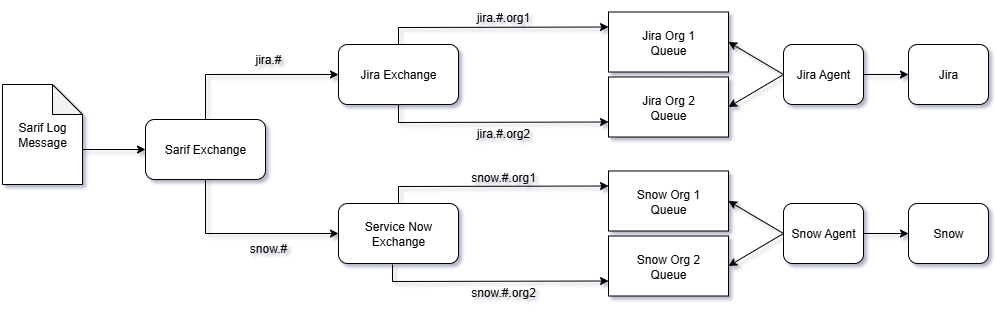
\includegraphics[width=\textwidth]{graphics/cxoneflow-diagrams-sarif-exchange-example.png}
    \caption{Sarif Log Delivery Example AMQP Schema}
    \label{fig:sarif-amqp-example}
\end{figure}


\subsection{HTTP Sarif Log Delivery}\label{sec:push-sarif-http}

HTTP delivery allows one or more HTTP endpoints to be defined where the Sarif log will be
POSTed.  The endpoint would receive the POST request and process the Sarif log as
appropriate.

Depending on the volume of scanning and production of Sarif logs, the implementation
of an HTTP receiver endpoint can be challenging.  If implementing a custom HTTP endpoint
receiver, the implementation should follow these guidelines:


\begin{itemize}
    \item When receiving the request, the response should be sent without waiting for
    a complete processing of the Sarif log.  A long delay before response will cause the
    sender to time out and attempt to retry the request.
    \item The receiver should persist the Sarif log for resuming workflows if the endpoint is terminated
    before all received Sarif logs are processed.
    \item The response status code when successfullying receiving a Sarif log should be a 2XX status.
    \item The response status code to a signature mismatch for the received message should be a 4XX status.
    \item The response status code to a failure to process the Sarif log should be a 5XX status.
\end{itemize}

The \cxoneflow delivery will retry on failure but otherwise the status codes are for logging purposes. 
If creating a custom HTTP receiver endpoint implementation is unstable or difficult, explore using
the AMQP delivery option.  The use of the AMQP integration will typically be easier given the difficult
implementation parts of an HTTP receiver endpoint are implemented by the queue fabric.

\subsection{Sender Verification with HMAC}
The method of authenticating the sender is to validate a signature hash calculated
from the body of the delivered message.  This is done using a secret value
known by both the sender and receiver.  There is no need for sender and receiver to
exchange the shared secret; the signature verification allows each side to demonstrate
knowledge of the shared secret by producing the same calculated signature for the
exchanged message content.

If the signature calculated by the receiver matches the signature sent
by the sender, it is verified the sender and receiver both know the same
shared secret.  If the signatures don't match, the received message is typically
discarded since the sender can't be verified by demonstrating knowledge of a
mutually shared secret.  The data integrity is also ensured given the signature
of the received body content would not have a matching signature if it was
modified in transit.

The signature is typically validated prior to processing the received contents.  This
allows data sent by unverified senders or data that was modified in transit to be
discarded.

Examples of signature verification are provided in the next section.
\footnote{Do not use the example shared secret in production; it is for demonstration purposes only.}

\subsubsection{AMQP HMAC Signature Verification Example}

The example code for demonstrating HMAC signature validation with an AMQP receiver
consumes a pre-defined queue that has been bound to a pre-defined exchange. Sarif logs are
delivered to the exchange and the queue is bound to the exchange.  Agents that consume
the queue are given messages from the queue to handle as appropriate.

The example reads the signature and algorithm from the received message headers.
The receiver, which also knows the shared secret used to calculate the signature
by the sender, recalculates the signature on the received message content.  If the signatures
match, the message is verified as sent by the correct sender.



\begin{code}{HMAC Signature Verification Example}{[AMQP]}{}
import hmac
import asyncio, aio_pika

# An example of how to verify the HMAC signature
# of the received Sarif log body.

async def receive_sarif_log(msg: aio_pika.abc.AbstractIncomingMessage) -> None:
    try:
       
      shared_secret = "MySharedSecret-12344$abc!123"
      sig = msg.headers['x-cx-signature']
      alg = msg.headers['x-cx-signature-alg']
      print(f"Received message with signature: {sig} generated using algorithm {alg}")

      h = hmac.new(bytes(shared_secret, 'UTF-8'), msg.body, alg)
      if h.hexdigest() != sig:
          print(f"Calculated signature {h.hexdigest()} is invalid.")
      else:
        print("The signature verified correctly.")

    except BaseException as ex:
        await msg.nack(requeue=False)
    finally:
        await msg.ack()

async def be_an_agent():
  mq_client = await aio_pika.connect_robust("amqp://localhost/sarif")
  async with mq_client.channel() as channel:
      q = await channel.get_queue("SARIF")
      await q.consume(receive_sarif_log)
      while True:
          await asyncio.Future()

if __name__ == "__main__":
  asyncio.run(be_an_agent())
\end{code}



\subsubsection{HTTP HMAC Signature Verification Example}

The example code for demonstrating HMAC signature validation with an HTTP receiver
is a simple Flask application. The application acts as an HTTP receiver endpoint
for receiving Sarif logs.  The example reads the signature and algorithm from the request
headers.  The receiver, which also knows the shared secret used to calculate the signature
by the sender, recalculates the signature on the received body content. If the signatures
match, the message is verified as sent by the correct sender.

\begin{code}{HMAC Signature Verification Example}{[HTTP]}{}
import hmac
from flask import Flask, request, Response

# An example of how to verify the HMAC signature
# of the received Sarif log body.

app = Flask("Example")

@app.route("/sarif", methods=['POST'])
async def validate__hmac_signature():
    shared_secret = "MySharedSecret-12344$abc!123"
    sig = request.headers['x-cx-signature']
    alg = request.headers['x-cx-signature-alg']
    print(f"Received message with signature: {sig} generated using algorithm {alg}")

    h = hmac.new(bytes(shared_secret, 'UTF-8'), request.data, alg)
    if h.hexdigest() != sig:
        print(f"Calculated signature {h.hexdigest()} is invalid.")
        return Response(status=403)
    else:
      print("The signature verified correctly.")
      return Response(status=204)

\end{code}


\subsection{Scan Error Message Delivery}

In the event of a scan error that prevents the generation of a Sarif log, a message is delivered with the header
\texttt{x-cx-is-error} set to True.  The HMAC validation of the content to confirm a valid sender can be
performed as it is with a message containing a Sarif log.

The body of the message when the \texttt{x-cx-is-error} header indicates the message is an error is a simple
JSON dictionary containing one key named \texttt{error}.  The value for \texttt{error} is a simple text string
indicating the reason for the failure.  The message headers will contain details of the scan parameters that
can be used to further query the SCM and \cxone if necessary.

